\documentclass[conference]{IEEEtran}
\IEEEoverridecommandlockouts
\usepackage{amsmath,amssymb}
\usepackage{booktabs}
\usepackage{url}
\usepackage{tikz}
\usepackage{pgfplots}
\pgfplotsset{compat=1.17}
\usetikzlibrary{arrows.meta,positioning}

\begin{document}

\title{Riptide: Breaking the Serial Window Chain in\\ Parallel Gzip Decompression}

\author{
\begin{tabular}{@{}c@{\hspace{2.2cm}}c@{}}
\textbf{Devansh Hiren Shah} & \textbf{Mantri Samarth Prakash}\\
Dept. of Information Technology & Dept. of Information Technology\\
NIT Karnataka, Surathkal --- 241IT024 & NIT Karnataka, Surathkal --- 241IT043\\[8pt]
\textbf{Shubh Minesh Thakkar} & \textbf{Ritesh Bhagat}\\
Dept. of Information Technology & Dept. of Information Technology\\
NIT Karnataka, Surathkal --- 241IT076 & NIT Karnataka, Surathkal --- 241IT063
\end{tabular}
}

\maketitle

\begin{abstract}
Decompressing a gzip file is a single-core task in standard tools, because DEFLATE
blocks have no index and back-references reach 32\,KiB into earlier output. The
two-stage scheme of \texttt{rapidgzip}, our base paper, decodes chunks in parallel
with placeholders for unknown bytes, but resolves the windows that fill them in one
chunk after another, a step the paper states cannot be parallelised. We show that
each chunk's window is a function of its predecessor's, that these functions compose
associatively, and that the chain is therefore a parallel prefix scan. We built
Riptide, a complete parallel gzip decoder written from scratch in C++20, with three
scan algorithms, a work-stealing runtime and an overflow policy that splits chunks
exceeding their memory budget across idle cores. On a 10-core Apple M4, all 1\,200
timed runs are byte-identical to zlib; Riptide decodes the Silesia corpus at
2.60\,GB/s and a 1\,GB Silesia file at 3.01\,GB/s, 2.1--2.5$\times$ zlib. The
blocked scan resolves windows 2.9--3.9$\times$ faster than the serial chain, which
makes the whole decompression up to 1.21$\times$ faster with small chunks, which use
up to 35\% less memory; with 4\,MiB chunks the chain is under 1\% of the run.
Splitting overflowing chunks lowers load imbalance from 5.6 to 1.3 and run time by
1.59$\times$ when there are few chunks per core, while header-driven work-balanced
chunking does not pay off.
\end{abstract}

\begin{IEEEkeywords}
gzip, DEFLATE, parallel decompression, prefix scan, work stealing, load balancing
\end{IEEEkeywords}

\section{Introduction}

Gzip is the most common compressed format for data that is written once and read
many times: sequencing reads (\texttt{.fastq.gz}), service logs, scientific archives
and the default codec of many data-lake tables. Compressing it parallelises easily,
because a compressor may cut its input anywhere. Decompressing one \texttt{.gz} file
does not: zlib, the reference decoder, uses one core, and widely used tools such as
\texttt{pigz} parallelise only reading and writing around a serial decode loop. A
genomics pipeline that aligns reads on dozens of cores, or a query engine that scans
a gzipped log, therefore waits on a single thread.

Two properties of DEFLATE~\cite{deflate} make the stream serial. Blocks are not
byte-aligned and the stream has no index, so a thread that starts at an arbitrary
offset does not know where a block begins. And a back-reference may copy bytes from
up to 32\,KiB earlier in the output, so a chunk can need data that an earlier chunk
has not produced yet. The two-stage scheme of \texttt{pugz}~\cite{pugz}, made general
and fast by \texttt{rapidgzip}~\cite{rapidgzip}, our base paper, handles both: threads
find block starts speculatively and decode chunks with \emph{markers} in place of the
unknown preceding bytes, which are filled in once those bytes are known.

The windows that fill in the markers are still computed one chunk after another,
and the base paper states that this propagation cannot be parallelised. We show that
it can. Each chunk's final window is a function of the window before it, these
functions compose associatively, and the chain is therefore a prefix scan. We also
revisit the base paper's handling of chunks that expand beyond their memory budget.

We implemented the complete decoder from scratch in C++20, about 5\,300 lines without
dependencies other than zlib for testing and comparison: a table-driven inflater,
speculative block finder, work-stealing thread pool, three parallel prefix scans,
parallel CRC-32 and the pipeline that connects them. Our contributions are:
\begin{itemize}
\item \textbf{M3 (primary):} window resolution by parallel prefix scan, replacing the
base paper's $N-1$ dependent steps with a blocked scan of span $O(P)$, evaluated
against Hillis--Steele and Blelloch scans.
\item \textbf{M1:} splitting chunks that exceed their output budget across idle
workers, and a work-balanced chunking policy driven by Huffman headers, which our
measurements show does not pay off.
\item A measured account of where the time and memory of two-stage decoding go, on
real and synthetic data, including the problems we had to fix to get there.
\end{itemize}

\section{Literature Survey}

\emph{Serial decoders.} zlib is the reference implementation of DEFLATE.
\texttt{libdeflate} and Intel ISA-L (\texttt{igzip}) make one thread faster with
wider bit buffers, larger tables and vector instructions, but do not use more
cores. \texttt{pigz} compresses in parallel but decompresses on one thread, with
separate threads only for reading, writing and the checksum.

\emph{Changing the format.} Formats that cut the stream into independently
compressed members, such as BGZF in genomics~\cite{samtools}, decompress in parallel
trivially, and index tools such as zlib's \texttt{zran} example or \texttt{gztool}
store windows at access points to allow random access. Both require the file to be
written differently or read sequentially once, which is the cost we want to avoid
for files that already exist.

\emph{Decoding unmodified gzip in parallel.} Kerbiriou and Chikhi~\cite{pugz}
observed that decoding symbols needs only the bit position and the block's Huffman
tables, and that the bytes copied from an unknown window can be represented by
placeholders; their \texttt{pugz} was limited to ASCII text. Knespel and
Brunst~\cite{rapidgzip} generalised the idea to arbitrary data in
\texttt{rapidgzip}: a fast block finder with a cheap pre-filter, speculative decoding
that is validated by chaining, a cache of prefetched chunks, and 16-bit output that
switches to 8 bits once markers can no longer occur. With 128 cores it reaches
5.6\,GB/s on Silesia, 33 times GNU gzip, but without an index its throughput stops
growing at about 64 cores, which the paper attributes to the sequential parts of
the pipeline, among them the window propagation. Its implementation also bounds each chunk's output, decoding
the rest of an oversized chunk on one thread~\cite{changelog}.

\emph{GPUs.} Sitaridi et al.~\cite{sitaridi} and Weißenberger and
Schmidt~\cite{weissenberger} decode Huffman and LZ77 data massively in parallel, but
on formats prepared for it, not on arbitrary gzip.

\emph{Parallel prefix and scheduling.} Hillis and Steele~\cite{hillis} gave the
step-efficient scan with $\lceil\log_2 N\rceil$ rounds and $O(N \log N)$ work;
Blelloch's~\cite{blelloch} up-sweep/down-sweep scan is work-efficient with $O(N)$
work and $2\lceil\log_2 N\rceil$ rounds. Both need only associativity, not
commutativity, which is what window composition provides. Our runtime follows the
randomised work-stealing scheme of Blumofe and Leiserson~\cite{blumofe}, with a deque
per worker as in Chase and Lev~\cite{chaselev}, although protected by a lock rather
than lock-free because our tasks are coarse.

\section{Methodology}

\subsection{Datasets}

The primary dataset is the Silesia corpus, the base paper's benchmark: twelve files
of 212\,MB in total, packed into one tarball and compressed with \texttt{gzip -6},
giving 68.2\,MB and an expansion ratio of 3.11 (the base paper reports 3.1). To
measure larger inputs and other regimes we generate four more files with fixed seeds
(Table~\ref{tab:data}): five copies of the Silesia tarball in one gzip member, as the
base paper scales its inputs; short-read FASTQ records; structured service logs that
compress more than 20$\times$, the regime in which the base paper's software
serialises; and a mixed archive that interleaves Silesia files with random data and
logs, so that expansion changes abruptly inside one stream. Every output is checked
byte for byte against zlib.

\begin{table}[t]
\caption{Datasets (measured)}
\label{tab:data}
\centering
\footnotesize
\setlength{\tabcolsep}{3pt}
\begin{tabular}{@{}llrr@{}}
\toprule
\textbf{File} & \textbf{Content} & \textbf{Output} & \textbf{Ratio} \\
\midrule
\texttt{silesia} & Silesia corpus tarball & 212\,MB & 3.11 \\
\texttt{silesia\_x5} & five copies, one member & 1.06\,GB & 3.11 \\
\texttt{reads} & synthetic 150\,bp FASTQ & 1.08\,GB & 4.11 \\
\texttt{logs} & synthetic JSON service logs & 1.08\,GB & 23.1 \\
\texttt{mixed} & Silesia, random data, logs & 444\,MB & 3.51 \\
\bottomrule
\end{tabular}
\end{table}

\subsection{Pipeline}

Fig.~\ref{fig:pipeline} shows the decoder. All stages except chain linking run on
one work-stealing pool.

\begin{figure*}[t]
\centering
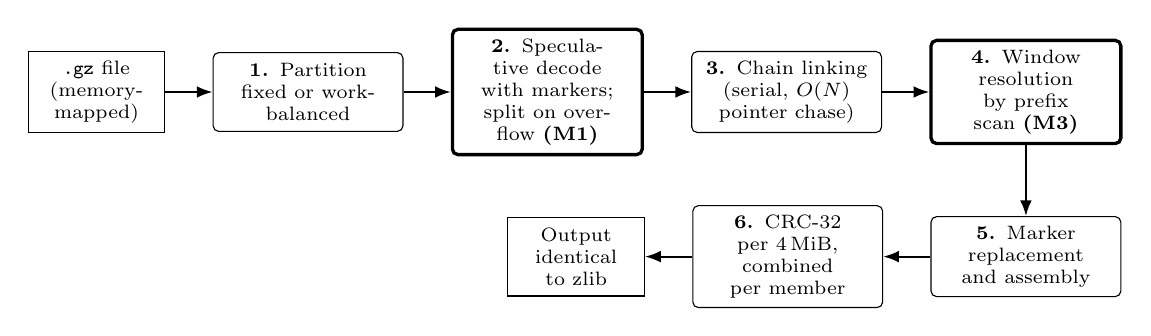
\begin{tikzpicture}[
  node distance=5mm and 6mm,
  box/.style={draw, rounded corners=2pt, align=center, font=\scriptsize,
              minimum height=10mm, inner xsep=3pt, text width=22mm},
  novel/.style={box, very thick},
  io/.style={draw, align=center, font=\scriptsize, minimum height=10mm, text width=15mm},
  a/.style={-{Latex[length=2mm]}, thick}
]
\node[io] (in) {\texttt{.gz} file\\ (memory-mapped)};
\node[box, right=of in] (part) {\textbf{1.} Partition\\ fixed or work-balanced};
\node[novel, right=of part] (dec) {\textbf{2.} Speculative decode\\ with markers;\\ split on overflow \textbf{(M1)}};
\node[box, right=of dec] (chain) {\textbf{3.} Chain linking\\ (serial, $O(N)$\\ pointer chase)};
\node[novel, right=of chain] (win) {\textbf{4.} Window resolution\\ by prefix scan \textbf{(M3)}};
\node[box, below=9mm of win] (rep) {\textbf{5.} Marker replacement\\ and assembly};
\node[box, left=of rep] (crc) {\textbf{6.} CRC-32 per 4\,MiB,\\ combined per member};
\node[io, left=of crc] (out) {Output identical\\ to zlib};
\draw[a] (in) -- (part);
\draw[a] (part) -- (dec);
\draw[a] (dec) -- (chain);
\draw[a] (chain) -- (win);
\draw[a] (win) -- (rep);
\draw[a] (rep) -- (crc);
\draw[a] (crc) -- (out);
\end{tikzpicture}
\caption{Riptide's pipeline. Bold stages contain our contributions; speculative
decoding with markers and the block finder follow the base paper.}
\label{fig:pipeline}
\end{figure*}

\emph{Speculative decoding.} The input is cut into chunks of equal compressed size.
A task searches its range for a block header: a 13-bit pre-filter (not final,
dynamic type, valid code counts) rejects 89\% of bit offsets, a check that the
code-length code is complete rejects nearly all others using one 64-bit load, and
the survivors have both Huffman codes read and validated. Stored blocks are found by
their length and its complement at a byte boundary. The task then decodes from that
block with a window of 32\,768 markers $\mathtt{0x8000}+j$ standing for the unknown
bytes, writing 16-bit symbols until the last 32\,KiB of output hold no marker, after
which it continues with 8-bit output. It stops at the first block boundary past the
next chunk's start.

\emph{Chain linking.} Starting from the first chunk, the next link is the chunk that
began exactly where the current one stopped. A chunk that began at a false-positive
header has no predecessor that stops there and is discarded; a missing link is
decoded on the spot.

\subsection{M3: Window Resolution by Prefix Scan}

After linking, the last 32\,KiB of every chunk $k$ is a vector of symbols, each a
byte or a marker into the window $W_{k-1}$ that chunk $k$ started with. It is
therefore a map $f_k$ with $W_k = f_k(W_{k-1})$. The base paper evaluates
$W_1 = f_1(W_0)$, $W_2 = f_2(W_1)$ and so on, $N-1$ dependent steps. Two maps compose
into a map of the same form, $(g \circ f)[i] = g[i]$ if $g[i]$ is a byte and
$f[j]$ if $g[i]$ is the marker $j$, a 32\,KiB gather. Composition of functions is
associative, so
\[
W_k = (f_k \circ f_{k-1} \circ \cdots \circ f_1)(W_0)
\]
is an inclusive prefix scan and any parallel scan applies. We implemented three. The
Hillis--Steele scan takes $\lceil\log_2 N\rceil$ rounds and about $N\log_2 N$
compositions; the Blelloch scan $2\lceil\log_2 N\rceil$ rounds and $O(N)$. The
blocked scan, which we use by default, splits the $N$ maps into $P$ contiguous blocks,
composes each block in parallel, resolves the $P$ block-entry windows in order, and
then applies each block's maps in parallel: about $2N$ compositions in three
phases, whose longest chain of dependent compositions is $2N/P + P$. On $P$ cores a
scan takes roughly its work divided by $P$ plus its span. Measured on $N = 5\,205$
chunks with $P = 10$, the serial chain performs 5\,204 dependent steps;
Hillis--Steele 14 rounds but 59\,461 compositions, about 5\,900 per core; Blelloch
28 rounds and 21\,586 compositions, as its down-sweep and the final application each
touch every element; and the blocked scan 10\,417 compositions with a longest
dependent chain of 1\,051. We use the blocked scan by default: it has the least work
per core, three synchronisation points instead of one per round, and phases that work
on contiguous chunks, which matters because a composition reads and writes 64\,KiB
and is memory-bound.

\subsection{M1: Output Budgets and Work-Balanced Chunks}

Every chunk has an output budget, by default 20 times its compressed size, which
bounds memory and stops speculative decoding from a false positive early. When a
chunk reaches its budget, the base paper's software decodes the rest of it on one
thread. With the \emph{split} policy we stop at the next block boundary and schedule
the remaining compressed range as up to $P$ speculative pieces that find their own
block starts; chain linking connects them, so correctness does not depend on where
the cuts fall. The \emph{work-balanced} policy samples a dynamic header every
512\,KiB, estimates bytes per symbol and expansion from its code lengths (a code of
length $L$ has probability about $2^{-L}$) and cuts chunks of equal estimated cost
instead of equal size.

\subsection{Runtime and Verification}

Each worker owns a deque, runs its own newest tasks first and steals the oldest
tasks of others. A task group waits by running pending tasks, so tasks that schedule
sub-tasks into their own group, as split-on-overflow does, cannot deadlock the pool.
Each worker records its busy time, from which we report the first-stage load
imbalance $\lambda$, the busiest worker's time over the mean. Marker replacement and
copying run as 1--4\,MiB pieces, and each chunk is released as soon as its last piece
is written. CRC-32 is computed per 4\,MiB block, with ARMv8 CRC instructions where
available, and block CRCs are joined by multiplying with $x^{8n}$ modulo the CRC
polynomial.

\subsection{Implementation and Testing}

The code base is organised by layer (bit reader, Huffman, inflate, gzip, parallel
runtime, windows, pipeline) and builds with CMake without a warning at
\texttt{-Wall -Wextra -Wpedantic -Wshadow -Wconversion}. 44 unit and integration tests compare
every chunk size, scan, policy, block type, compression level and multi-member file
with zlib and check that corrupted and truncated streams are rejected; they run
clean under AddressSanitizer, UndefinedBehaviorSanitizer and ThreadSanitizer.

\emph{Problems we had to solve.} A task group could be destroyed while the worker
that completed its last task was still notifying it, which failed in one run in
eight until the decrement and notification were made under the group's mutex.
Decoding a truncated stream looped forever, because the bit reader returns zeros
past the end and zeros decode as literals. The block finder initially zero-filled
full Huffman tables for every candidate. Our first complete benchmark run then
exposed two more: the decoder used 7.6\,GB to decompress the 1\,GB log file, because
growing vectors were zero-filled and kept their capacity and every chunk stayed
alive until assembly ended; and the finder scanned incompressible regions bit by bit
for dynamic headers that were not there, making the parallel decoder on one thread
2.5$\times$ slower than the sequential one on the mixed archive. Fixing them halved
the time and memory on the log file and made the mixed archive 3.6$\times$ faster.
Finally, the benchmark itself ran each configuration's repetitions back to back, and
on our fanless test machine the same configuration measured 48\% slower ten minutes
later; all results below interleave repetitions across configurations.

\section{Results}

\subsection{Experimental Setup}

All experiments ran on an Apple M4 with 4 performance and 6 efficiency cores and
16\,GB of memory, under macOS 27.0.1, compiled with Apple clang 21 at \texttt{-O3}.
Each configuration ran once unmeasured and 10 times measured, with repetitions
interleaved round-robin across all configurations of a file. We report medians;
configurations are compared with the two-sided Mann--Whitney U
test~\cite{mannwhitney}, since repeated runs are independent samples rather than
pairs, with Holm--Bonferroni correction~\cite{holm} over all comparisons of an
experiment. The baselines are zlib and Riptide's own sequential decoder, which uses
the same inflate code with a known window.

\subsection{Correctness}

All 1\,200 timed runs, across five files, six thread counts, seven chunk sizes, four
scans and four policy combinations, produced output byte-identical to zlib.

\subsection{Scaling}

\begin{figure}[t]
\centering
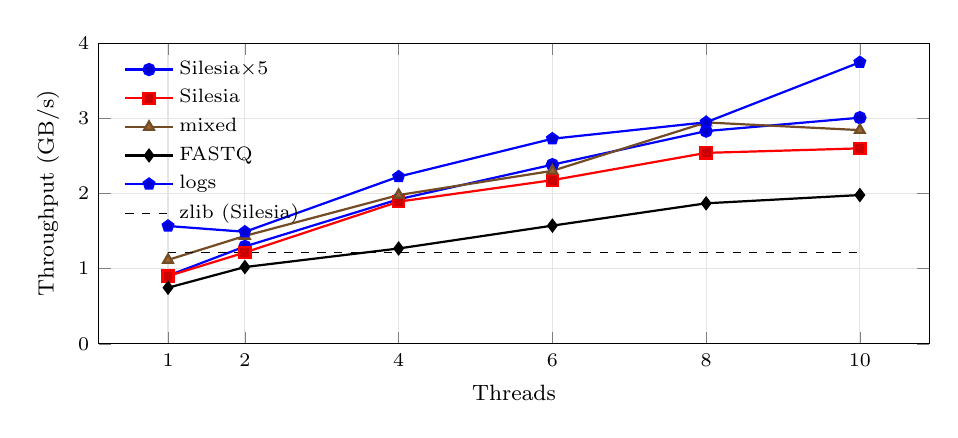
\begin{tikzpicture}
\begin{axis}[
  width=\columnwidth, height=5.4cm,
  xlabel={Threads}, ylabel={Throughput (GB/s)},
  xtick={1,2,4,6,8,10}, ymin=0, ymax=4,
  legend style={font=\scriptsize, at={(0.02,0.98)}, anchor=north west, draw=none, fill=none},
  legend cell align=left, tick label style={font=\scriptsize}, label style={font=\footnotesize},
  grid=major, grid style={gray!20}]
\addplot+[mark=*, thick] coordinates {(1,0.906) (2,1.295) (4,1.923) (6,2.383) (8,2.830) (10,3.008)};
\addplot+[mark=square*, thick] coordinates {(1,0.901) (2,1.215) (4,1.891) (6,2.177) (8,2.540) (10,2.600)};
\addplot+[mark=triangle*, thick] coordinates {(1,1.116) (2,1.435) (4,1.979) (6,2.301) (8,2.945) (10,2.843)};
\addplot+[mark=diamond*, thick] coordinates {(1,0.746) (2,1.021) (4,1.268) (6,1.572) (8,1.869) (10,1.979)};
\addplot+[mark=pentagon*, thick] coordinates {(1,1.567) (2,1.490) (4,2.224) (6,2.728) (8,2.947) (10,3.745)};
\addplot[dashed, black, domain=1:10] {1.216};
\legend{Silesia$\times$5, Silesia, mixed, FASTQ, logs, zlib (Silesia)}
\end{axis}
\end{tikzpicture}
\caption{Throughput against threads, 4\,MiB chunks, blocked scan (median of 10).
The log file's zlib throughput, 6.04\,GB/s, is outside the plot.}
\label{fig:scaling}
\end{figure}

\begin{table}[t]
\caption{Throughput with 10 threads, 4\,MiB chunks (measured)}
\label{tab:scaling}
\centering
\footnotesize
\setlength{\tabcolsep}{3pt}
\begin{tabular}{@{}lrrrrr@{}}
\toprule
\textbf{File} & \textbf{zlib} & \textbf{Seq.} & \textbf{Riptide} & \textbf{vs zlib} & $\boldsymbol{S_{10}}$ \\
 & GB/s & GB/s & GB/s & & \\
\midrule
Silesia & 1.22 & 0.69 & 2.60 & 2.14 & 2.89 \\
Silesia$\times$5 & 1.22 & 0.69 & 3.01 & 2.47 & 3.32 \\
mixed & 1.93 & 0.93 & 2.84 & 1.47 & 2.55 \\
FASTQ & 1.64 & 0.85 & 1.98 & 1.21 & 2.65 \\
logs & 6.04 & 2.47 & 3.75 & 0.62 & 2.39 \\
\bottomrule
\end{tabular}
\end{table}

Fig.~\ref{fig:scaling} and Table~\ref{tab:scaling} show throughput; $S_{10}$ is the
speedup over Riptide on one thread. With 10 threads Riptide is 2.1--2.5$\times$
faster than zlib on Silesia and 4.4$\times$ faster than its own sequential decoder
on Silesia$\times$5. Our inflate loop is slower than zlib's (0.69 against
1.22\,GB/s), so roughly the first two cores only make up for that. Efficiency at
10 threads is about 0.3, for two reasons we can measure. The six efficiency cores
contribute less than the performance cores, so the curves bend after four threads.
And two-stage decoding adds work that a sequential decoder does not do: on
Silesia$\times$5 with one thread, decoding takes 922\,ms and marker replacement
another 188\,ms. On the log file 94\% of the output consists of markers, because
nearly every string is copied from earlier text that itself came from the unknown
window; replacement takes 145 of 288\,ms with 10 threads, and zlib, whose work there
is mostly long memory copies, stays faster. For reference, the base paper reports
5.6\,GB/s on Silesia with 128 cores~\cite{rapidgzip}; the machines are too different
for a direct comparison, and we did not run its code.

\subsection{M3: Window Resolution}

\begin{table}[t]
\caption{Window resolution on Silesia$\times$5, 10 threads (measured, ms)}
\label{tab:m3}
\centering
\footnotesize
\setlength{\tabcolsep}{2.6pt}
\begin{tabular}{@{}rrrrrrrr@{}}
\toprule
 & & \multicolumn{4}{c}{\textbf{Window step}} & \multicolumn{2}{c}{\textbf{Total}} \\
\cmidrule(lr){3-6}\cmidrule(l){7-8}
\textbf{Chunk} & $\boldsymbol{N}$ & \textbf{Serial} & \textbf{H--S} & \textbf{Blell.} & \textbf{Block.} & \textbf{Serial} & \textbf{Block.} \\
\midrule
64\,KiB & 5205 & 270.8 & 184.2 & 135.8 & 81.6 & 1258 & 1102 \\
128\,KiB & 2603 & 140.0 & 74.3 & 61.6 & 38.8 & 952 & 879 \\
256\,KiB & 1302 & 66.7 & 29.0 & 26.8 & 19.9 & 790 & 765 \\
512\,KiB & 651 & 28.3 & 11.0 & 11.3 & 7.2 & 680 & 656 \\
1\,MiB & 326 & 10.6 & 4.4 & 4.5 & 3.1 & 598 & 594 \\
2\,MiB & 163 & 4.2 & 2.2 & 2.2 & 1.3 & 532 & 529 \\
4\,MiB & 82 & 1.7 & 1.2 & 1.3 & 0.6 & 482 & 479 \\
\bottomrule
\end{tabular}
\end{table}

Table~\ref{tab:m3} shows the window step for all four strategies. The blocked scan
is 2.9--3.9$\times$ faster than the serial chain at every chunk size, and Blelloch
and Hillis--Steele fall in between. All
blocked-versus-serial differences in the window step are significant
($p < 0.001$ after correction). Whether this matters for the whole run depends on the
number of chunks. With 64\,KiB chunks the serial chain takes 22\% of the run, and the
scan makes the decompression 1.14$\times$ faster on Silesia$\times$5 and
1.21$\times$ on Silesia (311 to 257\,ms); at 128\,KiB the gains are 1.08$\times$ and
1.11$\times$. From 1\,MiB up the chain is under 2\% of the run and the totals do not
differ significantly. With 64\,KiB chunks and a varying thread count, the serial
chain costs 183--261\,ms regardless of threads, while the blocked scan falls from
221\,ms with 2 threads to 74\,ms with 10, 3.5$\times$ faster; with one thread it is
2$\times$ slower, since it does twice the work.

This bounds what M3 can give. With chunks of a few MiB the serial chain is
negligible, and our measurements do not support the idea that it
alone explains the base paper's scaling limit. It becomes significant when chunks are
small relative to the file, which is what one wants to save memory: 512\,KiB chunks
need 19\% less peak memory than 4\,MiB on Silesia$\times$5 (1.90 against 2.34\,GB)
and 35\% less on the log file (2.09 against 3.21\,GB). M3 removes most of the cost
that otherwise grows with the number of chunks.

\subsection{M1: Overflow and Chunking Policies}

\begin{table}[t]
\caption{Overflow policies, 10 threads, 4$\times$ output budget (measured)}
\label{tab:m1}
\centering
\footnotesize
\setlength{\tabcolsep}{3pt}
\begin{tabular}{@{}llrrr@{}}
\toprule
\textbf{File, chunk} & \textbf{Overflow} & \textbf{Total (ms)} & $\boldsymbol{\lambda}$ & \textbf{Ratio} \\
\midrule
logs, 16\,MiB & serial & 407.0 & 5.58 & \\
logs, 16\,MiB & split & 255.7 & 1.29 & 1.59$^{*}$ \\
logs, 4\,MiB & serial & 259.4 & 1.11 & \\
logs, 4\,MiB & split & 263.2 & 1.04 & 0.99 \\
Silesia$\times$5, 16\,MiB & serial & 414.2 & 1.20 & \\
Silesia$\times$5, 16\,MiB & split & 397.2 & 1.13 & 1.04 \\
\bottomrule
\multicolumn{5}{@{}l}{\scriptsize $^{*}$ $p < 0.001$ after correction; other differences not significant.}
\end{tabular}
\end{table}

Table~\ref{tab:m1} shows when splitting matters. With 16\,MiB chunks and a budget of
four times the chunk size, the log file has three chunks for ten threads, and the
serial policy turns each into a chain of continuations: $\lambda = 5.6$. Splitting
brings $\lambda$ to 1.3 and makes the run 1.59$\times$ faster. With 4\,MiB chunks
there are many more chunks than threads, the continuations of different chunks
already run in parallel, and splitting makes no significant difference; on Silesia
the budget is rarely reached.

Work-balanced chunking is a negative result. Sampling headers costs 10--74\,ms, and
the decode stage does not get faster: on the mixed archive $\lambda$ falls from 1.53
to 1.34, but decode time stays at 103--108\,ms because it is set by individual large
chunks, not by the plan. Totals are 0.65--0.91$\times$ those of fixed chunks. With
enough chunks per thread, work stealing already balances the load.

\subsection{Threats to Validity}

The test machine is a fanless laptop that lowers its clock under sustained load;
before we interleaved repetitions, the same configuration measured up to 48\% slower
ten minutes later, and the reported numbers are sustained rather than peak
throughput. All results come from one machine with heterogeneous cores. Three of the
five datasets are synthetic, though seeded and reproducible. The base paper's code
was not run, so comparisons with it rest on its published numbers.

\section{Conclusion and Future Scope}

The window chain of two-stage gzip decompression is a prefix computation, not an
inherently sequential one: window maps compose associatively, and a blocked parallel
scan resolves them 2.9--3.9$\times$ faster than the chain on 10 cores. The gain
matters exactly when chunks are small, which is also when decompression uses the
least memory, and it is negligible with chunks of a few MiB. Splitting
oversized chunks removes the serialisation that output budgets cause when there are
few chunks per core, while a header-driven plan is not worth its sampling cost. We
built the whole decoder from scratch, and much of the work went into problems the
measurements exposed: a use-after-free race in task groups, a hang on truncated
input, a block search that crawled through incompressible data, and peak memory of
seven times the output, which we reduced to under three.

Several directions remain. Marker replacement, not window resolution, is now the
largest parallel overhead on highly compressible data; storing runs of markers as
spans instead of 16-bit symbols (M2) would shrink the 16-bit data by 9--23\% on our
files, by our measurements, and reduce the data replacement has to read.
Streaming the output in order instead of assembling it in memory would bound memory
by the number of chunks in flight. Porting M3 into rapidgzip would test it on 64 to
128 cores, where the base paper sees its limit. Finally, window composition is a
gather over 32\,KiB and maps naturally onto GPUs, which could resolve thousands of
small chunks at once.

\begin{thebibliography}{00}
\bibitem{rapidgzip} M. Knespel and H. Brunst, ``Rapidgzip: Parallel decompression and seeking in gzip files using cache prefetching,'' in \emph{Proc. 32nd Int. Symp. High-Performance Parallel and Distributed Computing (HPDC '23)}, Orlando, FL, USA, 2023, doi: 10.1145/3588195.3592992.
\bibitem{pugz} M. Kerbiriou and R. Chikhi, ``Parallel decompression of gzip-compressed files and random access to DNA sequences,'' in \emph{Proc. IEEE Int. Parallel and Distributed Processing Symp. Workshops (IPDPSW)}, 2019, pp. 209--217, doi: 10.1109/IPDPSW.2019.00042.
\bibitem{deflate} P. Deutsch, ``DEFLATE compressed data format specification version 1.3,'' RFC 1951, 1996, doi: 10.17487/RFC1951.
\bibitem{changelog} M. Knespel, ``rapidgzip changelog,'' versions 0.6.0--0.16.0, 2023--2025. [Online]. Available: \url{https://github.com/mxmlnkn/rapidgzip/blob/main/CHANGELOG.md}
\bibitem{samtools} H. Li \emph{et al.}, ``The Sequence Alignment/Map format and SAMtools,'' \emph{Bioinformatics}, vol. 25, no. 16, pp. 2078--2079, 2009.
\bibitem{sitaridi} E. Sitaridi, R. Mueller, T. Kaldewey, G. Lohman, and K. A. Ross, ``Massively-parallel lossless data decompression,'' in \emph{Proc. 45th Int. Conf. Parallel Processing (ICPP)}, 2016, pp. 242--247.
\bibitem{weissenberger} A. Weißenberger and B. Schmidt, ``Massively parallel Huffman decoding on GPUs,'' in \emph{Proc. 47th Int. Conf. Parallel Processing (ICPP)}, 2018.
\bibitem{hillis} W. D. Hillis and G. L. Steele, ``Data parallel algorithms,'' \emph{Commun. ACM}, vol. 29, no. 12, pp. 1170--1183, 1986.
\bibitem{blelloch} G. E. Blelloch, ``Prefix sums and their applications,'' School of Computer Science, Carnegie Mellon University, Tech. Rep. CMU-CS-90-190, 1990.
\bibitem{blumofe} R. D. Blumofe and C. E. Leiserson, ``Scheduling multithreaded computations by work stealing,'' \emph{J. ACM}, vol. 46, no. 5, pp. 720--748, 1999.
\bibitem{chaselev} D. Chase and Y. Lev, ``Dynamic circular work-stealing deque,'' in \emph{Proc. 17th ACM Symp. Parallelism in Algorithms and Architectures (SPAA)}, 2005, pp. 21--28.
\bibitem{mannwhitney} H. B. Mann and D. R. Whitney, ``On a test of whether one of two random variables is stochastically larger than the other,'' \emph{Ann. Math. Statist.}, vol. 18, no. 1, pp. 50--60, 1947.
\bibitem{holm} S. Holm, ``A simple sequentially rejective multiple test procedure,'' \emph{Scand. J. Statist.}, vol. 6, no. 2, pp. 65--70, 1979.
\end{thebibliography}

\end{document}
